\documentclass{ximera}


%%%\colorlet{penColor}{blue!50!black} % Color of a curve in a plot
%\colorlet{gridColor}{gray!50} % Color of grid in a plot
%\colorlet{background}{white} % Color of the page
\newcommand{\ddx}{\frac{d}{dx}}
\newcommand{\dydx}{\frac{dy}{dx}}
\newcommand{\dd}[2][]{\frac{d #1}{d #2}}


\outcome{Interpret real-word examples of limits via average velocity
  and instantaneous velocity}

\outcome{Interpert the slope of secant lines verses the slope of
  tangent lines.}

\outcome{Using a graph to compute limits.}

\title{The idea of limits}

\begin{document}

\begin{abstract}
  This activity will motivate the need for limits in mathematics.
\end{abstract}
\maketitle

Limits appear in real world settings. In fact, your GPS device (or
phone) can use limits to estimate your velocity by computing
\textit{average velocity} on small time frames. You've known how to
compute average velocity for some time, it is just
\[
\text{average velocity} = \frac{\text{distance}}{\text{time}}.
\]
However, we are typically more interested in velocity at a specific
instant. This is called \textit{instantaneous velocity}. What does
this have to do with limits? 
\begin{center}
  \textbf{Instantaneous velocity is the limit of average velocity as the time frame goes to zero.} 
\end{center}



Let's use these ideas to analyze some data. On the 12th of April in
1961, the Soviet Union launched Yuri Gagarin into space. Gagarin became
first human to orbit the Earth. Not to be outdone, less than one month
later the United States launched Alan Shepard into space. However, not
only was Shepard's flight second, it was also \textit{suborbital},
meaning he did not orbit the Earth. Shepard's flight went up and then
came back down and the entire flight was less than 16 minutes
long. Nevertheless, the plot of Shepard's flight is ripe for analysis
via average velocity. Using data from \textit{Conference on Results of
  the First U.S. Manned Suborbital Space Flight (1961 : Washington,
  D.C.)}, we have constructed a plot of Alan Shepard's altitude over
time:

\begin{image}
  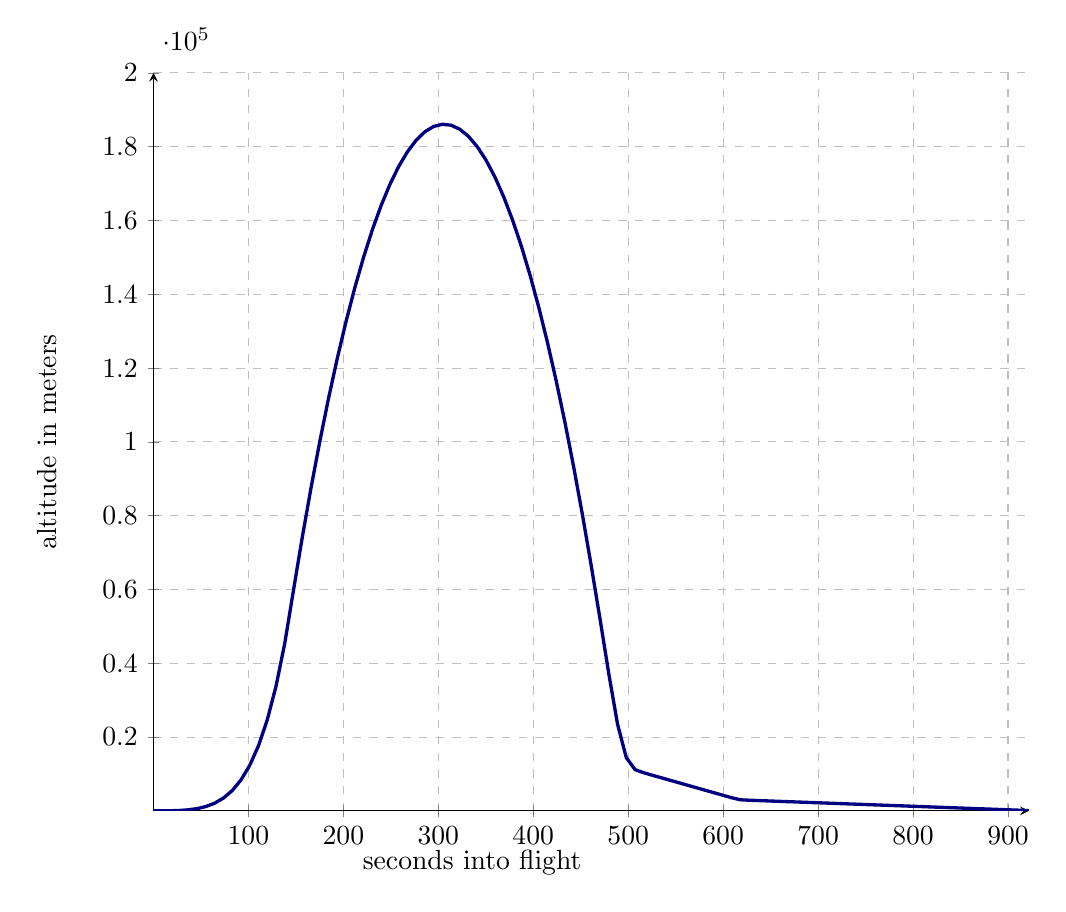
\begin{tikzpicture}
    \begin{axis}[
        xmin=0,
        xmax=922,
        ymin=0,
        ymax=200000,
        width=5in,
        axis lines=middle,
        y label style={at={(axis description cs:-0.1,0.5)},rotate=90,anchor=south},
        x label style={at={(axis description cs:0.5,-0.1)}},
        xlabel=seconds into flight, ylabel=altitude in meters,
        %xtick={0,1,...,12},
        %xticklabels={7am,8am,9am,10am,11am,12pm,1pm,2pm,3pm,4pm,5pm,6pm,7pm},
        %ytick={0,50,...,600},
            grid=both,
            grid style={dashed, gray!50},
      ]
      \addplot[very thick, blue!50!black] coordinates {
        (0.,0.) (9.222,4.35149) (18.444,34.812) (27.666,117.491) (36.888,288.148) (46.11,616.274) (55.332,1180.5) (64.554,2089.76) (73.776,3478.94) (82.998,5510.86) (92.22,8390.54) (101.442,12349.1) (110.664,17661.7) (119.886,24676.3) (129.108,33790.) (138.33,45456.6) (147.552,59899.1) (156.774,74172.4) (165.996,87586.9) (175.218,100143.) (184.44,111841.) (193.662,122682.) (202.884,132666.) (212.106,141794.) (221.328,150065.) (230.55,157481.) (239.772,164043.) (248.994,169749.) (258.216,174602.) (267.438,178602.) (276.66,181748.) (285.882,184042.) (295.104,185484.) (304.326,186074.) (313.548,185814.) (322.77,184702.) (331.992,182741.) (341.214,179930.) (350.436,176270.) (359.658,171762.) (368.88,166405.) (378.102,160201.) (387.324,153150.) (396.546,145252.) (405.768,136508.) (414.99,126918.) (424.212,116483.) (433.434,105203.) (442.656,93079.6) (451.878,80119.5) (461.1,66382.6) (470.322,51985.6) (479.544,37176.3) (488.766,23498.9) (497.988,14413.6) (507.21,11177.5) (516.432,10324.1) (525.654,9638.7) (534.876,8965.4) (544.098,8292.11) (553.32,7618.83) (562.542,6945.54) (571.764,6272.25) (580.986,5598.97) (590.208,4925.68) (599.43,4252.39) (608.652,3579.11) (617.874,3006.53) (627.096,2885.05) (636.318,2797.39) (645.54,2709.74) (654.762,2622.09) (663.984,2534.44) (673.206,2446.79) (682.428,2359.11) (691.65,2271.48) (700.872,2183.84) (710.094,2096.18) (719.316,2008.52) (728.538,1920.87) (737.76,1833.21) (746.982,1745.57) (756.204,1657.93) (765.426,1570.26) (774.648,1482.61) (783.87,1395.03) (793.092,1307.29) (802.314,1219.66) (811.536,1132.12) (820.758,1044.35) (829.98,957.081) (839.202,869.069) (848.424,781.391) (857.646,693.729) (866.868,606.152) (876.09,518.429) (885.312,430.782) (894.534,343.151) (903.756,255.466) (912.978,167.844) (922.2,80.1685)
      };
    \end{axis}
  \end{tikzpicture}
\end{image}

Alan Shepard's flight reached apogee (its highest point) around 300
seconds into the flight.

\begin{question}
  What was Alan Shepard's average velocity between the times of $0$ and
  $300$ seconds into his flight?
  \begin{multipleChoice}
    \choice[correct]{Around 600 meters per second.}
    \choice{Around $1.8$ meters per second.}
    \choice{Around $180000$ meters per second.}
    \choice{Around $300$ meters per second.}
    \choice{Impossible to estimate from the given information.}
  \end{multipleChoice}  
\end{question}

Around 500 seconds into the flight, Alan Shepard's capsule reentered
the atmosphere. This slowed the speed of the capsule considerably.

\begin{question}
  What was Alan Shepard's instantaneous velocity between the times of
  $500$ and $600$ seconds into his flight?
  \begin{multipleChoice}
    \choice[correct]{Around $-50$ meters per second.}
    \choice{Around $50$ meters per second.}
    \choice{Around $500$ meters per second.}
    \choice{Around $-500$ meters per second.}
    \choice{Impossible to estimate from the given information.}
  \end{multipleChoice}
\end{question}

Now let's look at this plot, where we have the altitude of Alan
Shepard's spacecraft along with a line:
\begin{image}
  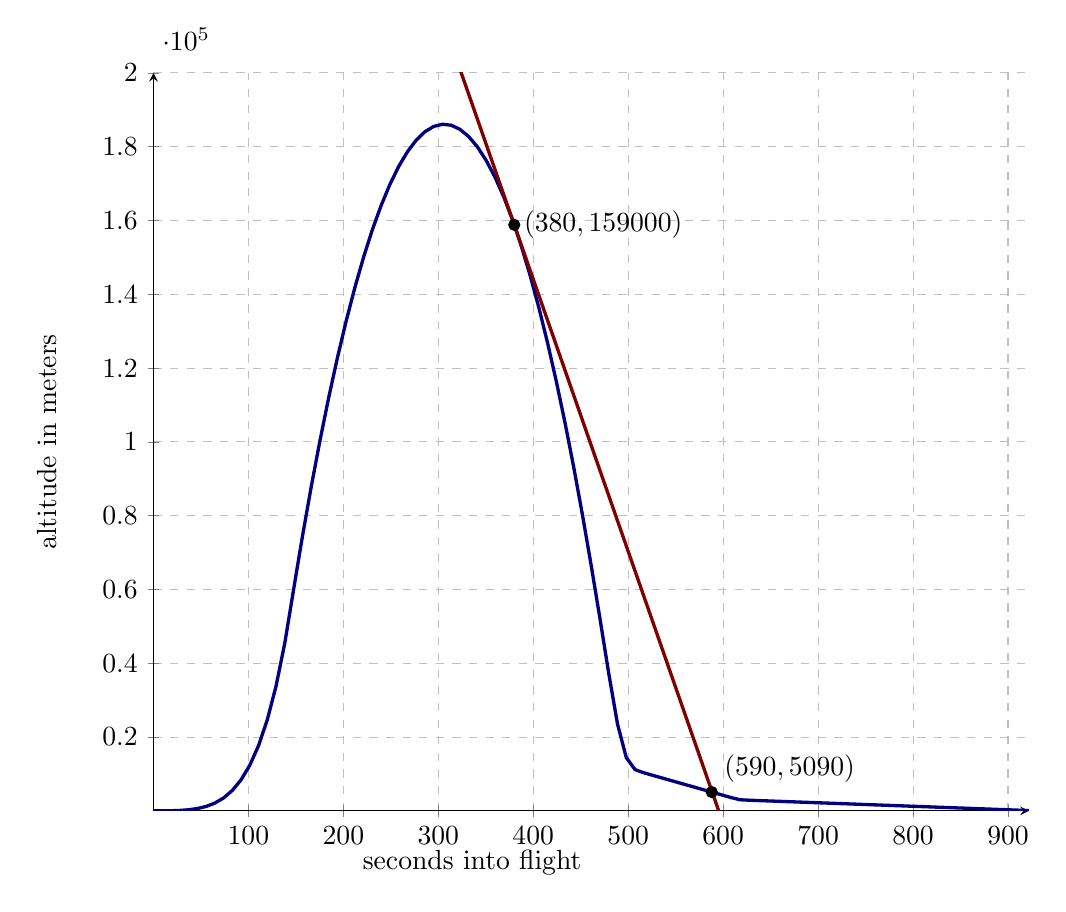
\begin{tikzpicture}
    \begin{axis}[
        domain=0:922,
        xmin=0,
        xmax=922,
        ymin=0,
        ymax=200000,
        width=5in,
        axis lines=middle,
        y label style={at={(axis description cs:-0.1,0.5)},rotate=90,anchor=south},
        x label style={at={(axis description cs:0.5,-0.1)}},
        xlabel=seconds into flight, ylabel=altitude in meters,
        %xtick={0,1,...,12},
        %xticklabels={7am,8am,9am,10am,11am,12pm,1pm,2pm,3pm,4pm,5pm,6pm,7pm},
        %ytick={0,50,...,600},
            grid=both,
            grid style={dashed, gray!50},
      ]
      \addplot[very thick, blue!50!black] coordinates {
        (0.,0.) (9.222,4.35149) (18.444,34.812) (27.666,117.491) (36.888,288.148) (46.11,616.274) (55.332,1180.5) (64.554,2089.76) (73.776,3478.94) (82.998,5510.86) (92.22,8390.54) (101.442,12349.1) (110.664,17661.7) (119.886,24676.3) (129.108,33790.) (138.33,45456.6) (147.552,59899.1) (156.774,74172.4) (165.996,87586.9) (175.218,100143.) (184.44,111841.) (193.662,122682.) (202.884,132666.) (212.106,141794.) (221.328,150065.) (230.55,157481.) (239.772,164043.) (248.994,169749.) (258.216,174602.) (267.438,178602.) (276.66,181748.) (285.882,184042.) (295.104,185484.) (304.326,186074.) (313.548,185814.) (322.77,184702.) (331.992,182741.) (341.214,179930.) (350.436,176270.) (359.658,171762.) (368.88,166405.) (378.102,160201.) (387.324,153150.) (396.546,145252.) (405.768,136508.) (414.99,126918.) (424.212,116483.) (433.434,105203.) (442.656,93079.6) (451.878,80119.5) (461.1,66382.6) (470.322,51985.6) (479.544,37176.3) (488.766,23498.9) (497.988,14413.6) (507.21,11177.5) (516.432,10324.1) (525.654,9638.7) (534.876,8965.4) (544.098,8292.11) (553.32,7618.83) (562.542,6945.54) (571.764,6272.25) (580.986,5598.97) (590.208,4925.68) (599.43,4252.39) (608.652,3579.11) (617.874,3006.53) (627.096,2885.05) (636.318,2797.39) (645.54,2709.74) (654.762,2622.09) (663.984,2534.44) (673.206,2446.79) (682.428,2359.11) (691.65,2271.48) (700.872,2183.84) (710.094,2096.18) (719.316,2008.52) (728.538,1920.87) (737.76,1833.21) (746.982,1745.57) (756.204,1657.93) (765.426,1570.26) (774.648,1482.61) (783.87,1395.03) (793.092,1307.29) (802.314,1219.66) (811.536,1132.12) (820.758,1044.35) (829.98,957.081) (839.202,869.069) (848.424,781.391) (857.646,693.729) (866.868,606.152) (876.09,518.429) (885.312,430.782) (894.534,343.151) (903.756,255.466) (912.978,167.844) (922.2,80.1685)
      };
      \addplot [very thick, red!50!black] {(x-380)*(-737.6)+158819};
      \addplot[color=black,fill=black,only marks,mark=*] coordinates{(380,158819)};
      \addplot[color=black,fill=black,only marks,mark=*] coordinates{(588,5086)};
      \node at (axis cs:380,158819) [anchor=west] {$(380,159000)$};
      \node at (axis cs:670,5100) [anchor=south] {$(590,5090)$};
    \end{axis}
  \end{tikzpicture}
\end{image}


\begin{question}
Viewing the line above as a \textbf{secant line}, which of the
following are true?
\begin{solution}
\begin{multiple-choice}
\choice[correct]{The average velocity on the interval from $380$ to $590$
  seconds into the flight is around $-733$ meters per second.}
\choice{The average velocity on the interval from $380$ to $590$
  seconds into the flight is around $733$ meters per second.}
\choice{The average velocity on the interval from $380$ to $590$
  seconds into the flight is around $0.0014$ meters per second.}
\choice{The average velocity on the interval from $380$ to $590$
  seconds into the flight is around $-0.0014$ meters per second.}
\end{multiple-choice}
\end{solution}
\end{question}


\begin{question}
Viewing the line above as a \textbf{tangent line}, which of the
following are true?
\begin{solution}
\begin{multiple-choice}
\choice[correct]{The instantaneous velocity at $380$
  seconds into the flight is around $-733$ meters per second.}
\choice{The instantaneous velocity at $380$
  seconds into the flight is around $733$ meters per second.}
\choice{The instantaneous velocity at $380$
  seconds into the flight is around $0.0014$ meters per second.}
\choice{The instantaneous velocity at $380$
  seconds into the flight is around $-0.0014$ meters per second.}
\end{multiple-choice}
\end{solution}
\end{question}


What other questions do you have about this lecture?
\begin{free-response}
Answers will vary.
\end{free-response}

\end{document}
